  \chapter{Výběr bezdrátové technologue pro senzorovou síť}
Navržená senzorová síť je napojena na infrastrukturu zavedeného přístupového systému v budově zákazníka s dosahem po celé budově a jejím okolí. Takto navržená síť umožní v těchto prostorách snímání dat z desítek senzorů.
Mezi hlavní kritéria pro vybranou bezdrátovou technologii patří nízká spotřeba energie koncových zařízení, nízká cena, jednoduchost implementace a možnost připojení koncových zařízení třetích stran.
Pro jednoduchost implementace vybraná bezdrátová technologie tedy musí používat pouze bezlicenční pásmo ISM a musí umožňovat uplementaci celé sítě bez závislosti na siti třetích stran. 


\section{Kandidátní bezdrátové technlogie}
Níže jsou popsány dostupné bezdrátové technologie vyhovující stanoveným kritériím pro tento projekt.

\begin{table}[]
  \begin{tabular}{|p{1.5cm}||p{2cm}|p{2cm}|p{2cm}|p{2cm}|p{2cm}|}
  \hline
  Technology    & topology options                & frequency bands  & range                                           & price per one transciever & availability of devices on the market \\ \hline \hline
  IQRF           & mesh, star                      & 868 MHz (Europe) & 10-100 m (in building), 100-1000 m (open space) & 15 – 20 \$                & very low                              \\ \hline
  wireless M-bus & star                            & 868M, 433M, 169M & 500 m (868 MHz), 2000 m (169 MHz)               & 25 – 30 \$                & low                                   \\ \hline
  ZigBee         & mesh, star                      & 2.4 GHz          & 100 m (open space)                              & 8 – 30 \$                 & high                                  \\ \hline
  BLE            & Point-to-Point, Broadcast, Mesh & 2.4 GHz          & 100 m (open space)                              & 5 – 20 \$                 & high                                  \\ \hline
  LoRa           & star                            & 868 MHz (Europe) & 15-22 km suburban, 3-8 km urban                 & 5 – 50 \$                 & medium                                \\ \hline
  Z-Wave         & mesh                            & 868 MHz (Europe) & 100 m in (open space), 30 m (in building)       & 10 – 50 \$                & high                                  \\ \hline
  Thread         & mesh                            & 2.4 GHz          & 100 m (open space)                              & 30 – 50 \$                & low                                   \\ \hline
  \end{tabular}
\end{table}

\subsection{IQRF}
IQRF je subGHz bezdrqátová technologie vyvinuta IQRF aliancí \cite{iqrf_alliance}, která je jediným výrobcem IQRF transceiveru \cite{iqrf_transceivers} za cenu v rozsahu \$15-20 za kus a k tomu poskytuje nástroje jako je SDK \cite{iqrf_sdk} a IDE \cite{iqrf_ide}. Z hlediska kriérií pro tento projekt je u této technologie nevýhodou nízký počet zařízení třetích stran dostupných na trhu. 
Většinou je tato technologie použita pro realizaci uživatelsé sítě, kde gateway je použita jedna z dostupných od IQRF aliance a koncová zařízení sítě jsou vytvořena vývojáři s použitím transceiverů od IQRF aliance
\cite{paper_iqrf}.


\section{Wireless M-bus}
Wireless M-Bus je standard specifikovaný v evropské normě EN 13757, popisující fyzickou, síťovou a aplikační vrstvu, původně navržen pro aplikace bezdrátového měření. 
Po několika letech v průmyslu bezdrátových měřících systémů se tato technologie rozšířila do oblasti průmyslu senzorových sítí.
Komunikace koncových zařízení je rozdělena do několika módů v závislosti na orientaci komunikace, objemu a vysílaných dat \cite{wirelessMBus01} \cite{wirelessMBus02}. Transceivery vyrábí více různých firem za cenu okolo \$25-30 za kus.


\section{Zigbee}
Zigbee je specifikace navržena pro IoT aplikace, založena na standardu  IEEE 802.15.4, vyvinuta Zigbee alliancí \cite{Zigbee_alliance}, vetšinou používána pro realizaci meshových sítí.
Dostupné transceivery na trhu se pohybují okolo \$8–30 od více různých výrobců, taktéž je i na trhu dostupnýchmnoho Zigbee koncových zařízení.


\section{BLE}
Bluetooth Low Energy (BLE) je verze Bluetooth s rádiem navrženým pro minimální spotřebu energie, umožňující topologie point-to-point, broadcast a mesh \cite{BT_alliance}.
Dostupné transceivery na trhu se pohybují okolo \$5–20 od více různých výrobců. Stejně tak je i na trhu mnoho dostupných koncových zařízení, ale mnohdy jsou tato koncová zařízení kompatibilní pouze se zařízení v rámci jednoho výrobce, tudíž může být problém je implementovat do vlastní senzorové sítě. 


\section{LoRa}
LoRa (Long Range) je modulace navržena firmou Semtech, LoRa Alliance vytvořila síťový protokol s názvem LoRaWAN postaven na fyzické vrstvě LoRa.
Protokol umožňuje ladit SF (Spreading Factor) neboli přenosovou rychlost, pro nastavení požadovaného dosahu \cite{lorawan_specification}.
V některých oblastech některé firmy poskytují pokrytí LoRaWAN sítí a proto je tato technologie velmi populární, Na trhu je mnoho koncových zařízení i gatewayí, s jejichž vzájemnou kompatibilitou neni problém. Gateway přeposílá přijaté packety s daty z koncových zařízení na server, kde je payload zpracován na základě dokumentace od výrobce daného koncového zařízení.
Semtech je jediným výrobcem integrovaných obvodů podporujících LoRa modulaci. Na trhu je dostupných mnoho transceiverů, které používají tento integrovaný obvod, některé dokonce obsahují implementovaný LoRaWAN stack.
Transceiver pro gateway má cenu okolo \$130 a umožňuje současně přijímat packety od koncových zařízení na více kanálech a přenosových rychlostech. Je zde i možnost udělat jednokanálovou gateway, která je schopna přijímat v jednu chvíli pouze jednom kanále a jedné přenosové rychlosti s použitím transceiveru pro koncová zařízení za cenu okolo \$5-30. V takové sítí pak musí být všechna koncová zařízení nakonfigurována na jednu konkrétní frekvenci a přenosovou rychlost.


% \begin{figure}[!h]
%     \centering
%     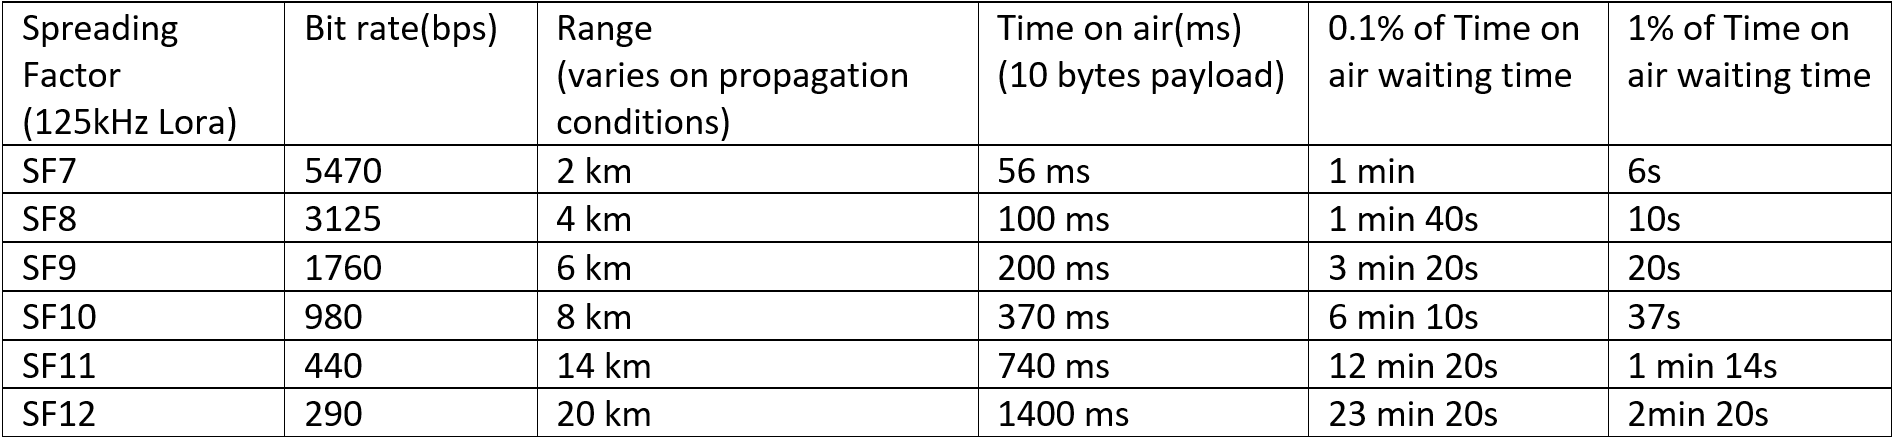
\includegraphics[width=1\textwidth]{spreading_factor_lorawan_2017-07-29}
%     \caption{LoRa spread factor options \cite{24}}
%     \label{fig:loraSF}
% \end{figure}

% \cite{19} \cite{20} \cite{21} \cite{22} \cite{23} \cite{24}.


\section{Z-Wawe}
Z-Wave is intended for wireless connectivity for all possible smart home products, controlled by PC, phone, voice, etc. It's based on mesh network topology so every non-battery powered device works as a router to enhance the network range so the more devices are connected in one network, the stronger the network is \cite{27} \cite{28}.


\section{Thread}
This technology based on IPv6 was developed for home network controlled by smartphone, tablet or PC \cite{29} \cite{30} \cite{31}.








\subsection{Wireless Sensor Network Design}
Wireless sensor network design is based on a popular IoT technology LoRa, which is a LPWAN technology using ISM band, 433 MHz, 868 MHz and 915 MHz (depends on the region) and communicates on multiple frequency channels and uses multiple data rates \cite{LoRaWAN Evaluation for IoT Communications}.
The LoRaWAN is an open standard network protocol and system architecture specified by \cite{LoRaWAN specification} and creates a media access control (MAC) layer on the top of the LoRa physical layer, secured by AES-128 encryption.
The LoRaWAN nodes communicate directly with the LoRaWAN gateway \cite{Internet of Things (IoT) using LoRa technology}.


